\section{Implementasi}

Bagian ini akan menjelaskan tentang implementasi sistem kontrol adaptif secara terperinci.

\subsection{Batasan Implementasi}
Berikut adalah batasan yang ditetapkan dalam melakukan implementasi sistem kontrol adaptif.
\begin{enumerate}
    \item Semua batasan masalah dan konfigurasi yang telah dibahas pada bagian \ref{sec:batasan-masalah}.
    \item Komponen \textit{Metrics Fetcher} berjalan di proses lain dan diimplementasikan dalam \textit{script} yang berbeda dikarenakan bahasa Python memiliki kekurangan dalam penanganan \textit{multithreading}.
    \item Pertukaran data antara komponen \textit{Metrics Fetcher} dan \textit{Predictor} melalui stream file.
\end{enumerate}

\subsection{Kakas yang Digunakan}
Dalam melakukan implementasi ini diperlukan beberapa kakas, diantaranya adalah sebagai berikut.
\begin{enumerate}
    \item \textit{Docker}, \textit{Docker Desktop} dan \textit{Docker Desktop Kubernetes} untuk dipakai sebagai \textit{containerization} dan \textit{cluster} kubernetes lokal.
    \item Pandas dan Numpy untuk keperluan \textit{data processing} serta bentuk data untuk dikirimkan ke komponen lain serta model prediksi ARIMA.
    \item \textit{Kubernetes Python Client} untuk mengontrol \textit{cluster} kubernetes melalui kode Python.
    \item \textit{Pickle} untuk menyimpan model ARIMA sehingga persisten meskipun sistem di-\textit{restart}.
    \item \textit{Statsmodels} dan \textit{pmdarima} untuk membangun model ARIMA serta melakukan otomasi pencarian orde atau lebih dikenal sebagai Auto-ARIMA.
\end{enumerate}

\subsection{Persiapan \textit{Pods Elastic Search}}

Sebelum melakukan implementasi, diperlukan untuk menyalakan \textit{Pods Elastic Search}. Konfigurasi ini dilakukan dengan cara membuat \textit{file deployment} untuk \textit{pods Elastic Search} serta sebuah \textit{persistent volume claim} untuk tempat penyimpanan data. Sebagai contoh dan konfigurasi yang dipakai dalam membuat tugas akhir ini dapat dilihat pada lampiran \ref{appendix:cth-konfigurasi-es-pods}.

\subsubsection{Komponen \textbf{\textit{Metrics Fetcher}}}
Seperti yang sudah dijelaskan sebelumnya, komponen ini akan menembak permintaan HTTP pada \textit{Node Stats API} (dokumentasi dapat dilihat pada tautan \url{https://www.elastic.co/guide/en/elasticsearch/reference/current/cluster-nodes-stats.html}) yang telah disediakan \textit{Elastic Search}. Komponen ini akan melakukan transformasi bentuk data menjadi lebih sederhana dan sesuai kebutuhan komponen lainnya. Khusus komponen ini, struktur kodenya tidak memakai sistem kelas dan hanya terdapat sebuah fungsi dan beberapa baris perintah untuk melakukan pemanggilan API, transformasi data dan pengiriman ke \textit{stream file}.
\subsection{Pengujian Komponen \textit{Predictor}}

Pada bagian ini akan dijelaskan tentang tujuan, skenario, hasil, dan analisis dari pengujian komponen \textbf{\textit{Predictor}}.

\subsubsection{Tujuan Pengujian}

Tujuan pengujian ini memastikan komponen \textbf{\textit{Predictor}} dapat berjalan dengan baik dan menghasilkan data yang sesuai dengan ekspektasi.

\subsubsection{Skenario Pengujian}

Pengujian terhadap komponen \textbf{\textit{Predictor}} dilakukan dengan membandingkan hasil prediksi dengan aktual untuk skenario sebagai berikut.
\begin{enumerate}
    \item \textit{Elastic Search} sedang \textit{idle}.
    \item \textit{Elastic Search} sedang digunakan untuk melakukan operasi penambahan data.
    \item \textit{Elastic Search} sedang digunakan untuk melakukan operasi pencarian data.
\end{enumerate}

\subsubsection{Hasil Pengujian dan Analisis}

% \begin{figure}[h]
%     \centering
%     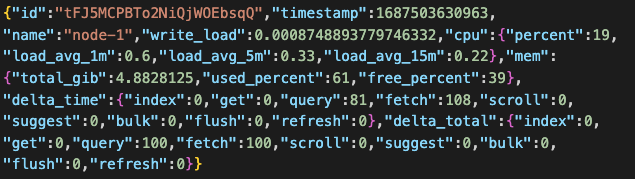
\includegraphics[width=0.8\textwidth]{chapter-4/mf-3.png}
%     \caption{Hasil Pengujian Komponen \textit{Metrics Fetcher} Skenario 3}
%     \label{fig:mf-3}
% \end{figure}

Pengujian komponen \textbf{\textit{Predictor}} menghasilkan angka yang cukup baik sehingga hasil prediksinya bisa dianggap merepresentasikan kondisi aktual.
\subsection{Komponen \textit{Rule Manager}}
Komponen \textbf{\textit{Rule Manager}} berfungsi untuk melakukan parsing terhadap file \textit{rule} yang telah diisi oleh pengguna serta menjadi aggregator untuk melakukan pengecekan \textit{rule} yang berlangsung serta memberi informasi data prediksi kapan saja yang dibutuhkan untuk melakukan pengecekan. Parsing komponen ini menggunakan format csv dan kondisi diekspresikan dengan sintaks python. Komponen akan mengonstruksi objek \textbf{\textit{Rule}} yang akan digunakan oleh komponen \textbf{\textit{Flexible Control}}. Agar terbayang, contoh dari \textit{file rule} dapat dilihat pada gambar \ref{fig:rule-example}. Spesifikasi dari kedua kelas tersebut dapat dilihat pada gambar \ref{fig:rule-spek}.

\begin{figure}[h]
    \centering
    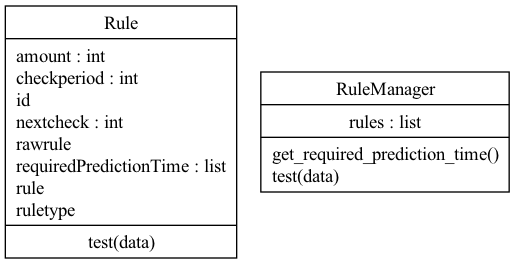
\includegraphics[width=0.8\textwidth]{chapter-4/rule.png}
    \caption{Spesifikasi Kelas Penyusun Komponen \textit{Rule Manager}}
    \label{fig:rule-spek}
\end{figure}

\begin{figure}[h]
    \centering
    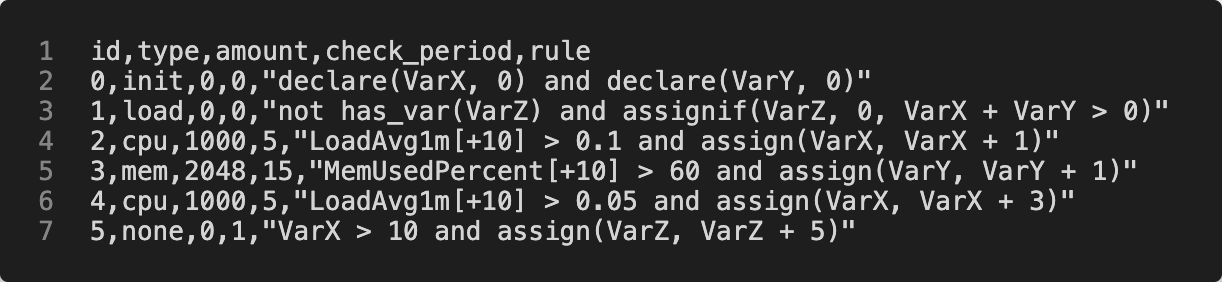
\includegraphics[width=0.75\textwidth]{chapter-4/cth-rule.png}
    \caption{Contoh \textit{File Rule}}
    \label{fig:rule-example}
\end{figure}

Sebuah \textit{rule} memiliki fungsi sebagai berikut.
\begin{enumerate}
    \item Memiliki sebuah kondisi yang akan dievaluasi dengan data prediksi pada waktu prediksi yang diinginkan. Contoh: kondisi \textit{throughput} untuk operasi X untuk 1 menit kedepan dan 5 menit kedepan lebih dari 1s, maka tingkatkan prosesor sebanyak 500m.
    \item Memiliki jumlah serta target kategori untuk diubah, dalam kasus ini pilihannya memori atau prosesor.
    \item Satuan untuk perubahan memori adalah dalam \textit{Mebibyte} atau MiB. Sedangkan untuk prosesor dalam satuan mili atau m.
    \item Sebuah \textit{rule} memiliki periode pengecekan sehingga tidak akan dicek secara terus menerus yang menyebabkan perubahan alokasi sumber daya terlalu cepat. Periode pengecekan dibuat dalam satuan sekon.
\end{enumerate}

Seperti yang bisa dilihat pada contoh gambar \ref{fig:rule-example}, untuk membuat sebuah \textit{rule}, terdapat 5 buah \textit{field} yang harus diisi. \textit{Field} tersebut adalah sebagai berikut.
\begin{enumerate}
    \item \textbf{ID}

        \textit{Field} ini dibebaskan kepada pengguna dan bertipe \textit{string} dan akan digunakan untuk mengidentifikasi \textit{rule} yang dibuat terutama jika terjadi error.
    \item \textbf{\textit{Type}}
    
        \textit{Field} ini bertipe \textit{string} dan akan digunakan untuk mengidentifikasi tipe eksekusi \textit{rule}. Berikut adalah pilihan yang dapat digunakan.
        \begin{enumerate}
            \item \textbf{\textit{Init}}
            
                \textit{Rule} akan otomatis berjalan diawal saat inisiasi (saat pertama kali dijalankan ataupun setelah di-\textit{reset}). Kategori pilihan ini digunakan untuk mendeklarasikan variabel \textit{user-defined} yang bisa digunakan untuk kondisi kompleks atau \textit{rule} yang saling berkaitan.

            \item \textbf{\textit{Load}}
            
                Berbeda dengan inisiasi, \textit{rule} ini akan berjalan ketika sistem dinyalakan dalam kondisi melanjutkan atau sesudah \textit{restart}. Kategori pilihan ini digunakan untuk mendeklarasikan variabel \textit{user-defined} yang mungkin ditambahkan saat \textit{restart}. Pada contoh gambar \ref{fig:rule-example}, dideklarasikan variabel $VarZ$ apabila belum terdefinisi dan $VarX+VarY > 0$.

            \item \textbf{\textit{None}}
            
                \textit{Rule} ini akan berjalan secara periodik namun tidak mengubah alokasi sumber daya apapun. Dapat digunakan untuk melakukan \textit{update} terhadap variabel \textit{user-defined}.

            \item \textbf{\textit{CPU}}

                Seperti namanya, digunakan untuk mengubah alokasi prosesor jika kondisi terpenuhi.
            \item \textbf{\textit{Mem}}
            
            Seperti namanya, digunakan untuk mengubah alokasi memori jika kondisi terpenuhi.
        \end{enumerate}

    \item \textbf{\textit{Amount}}
    
        \textit{Field} ini hanya berguna apabila tipe \textit{rule} adalah \textbf{CPU} atau \textbf{Mem}. Seperti namanya, digunakan untuk mengatur jumlah perubahan. Untuk \textbf{CPU}, angka dalam satuan milli. Sedangkan, untuk \textbf{Mem}, angka dalam satuan \textit{Mebibyte} (MiB).
    
    \item \textbf{\textit{Check Period}}
        
        \textit{Field} ini digunakan untuk mengatur periode pengecekan dalam satuan sekon. Periode ini berfungsi sebagai \textit{cooldown} jika kondisi bernilai benar. Setiap \textit{rule} yang ada akan dicek secara global setiap sekon, namun jika sudah bernilai benar, akan memasuki periode tidak dicek sampai periode pengecekan selesai. Jika kondisi bernilai salah, maka akan dicek kembali pada detik berikutnya. Tidak berlaku untuk tipe \textbf{init} dan \textbf{load} karena dua tipe tersebut akan selalu dijalankan sekali pada saat inisiasi atau \textit{restart}.

    \item \textbf{\textit{Rule}}
        
        \textit{Field} ini berisikan kondisi yang akan dievaluasi. Kondisi ini harus berupa ekspresi boolean yang terdiri dari variabel \textit{user-defined}, variabel prediksi metrik sistem dan operator logika. Variabel \textit{user-defined} dapat berupa variabel yang dideklarasikan pada \textit{rule} dengan tipe \textbf{init} atau \textbf{load} atau variabel yang dideklarasikan pada \textit{rule} lainnya. Operator logika yang dapat digunakan adalah \textbf{and}, \textbf{or}, dan \textbf{not}. Untuk operator perbandingan yang dapat digunakan adalah \textbf{$==$}, \textbf{$!=$}, \textbf{$>$}, \textbf{$>=$}, \textbf{$<$}, dan \textbf{$<=$}. Untuk operator aritmatika yang dapat digunakan adalah \textbf{+}, \textbf{-}, \textbf{*}, \textbf{/}, dan \textbf{\%}.

        Terdapat batasan berupa tidak bisa meletakkan variabel prediksi metrik sistem pada \textit{rule} bertipe \textbf{init} dan \textbf{load}. Apabila ingin menggunakan variabel prediksi metrik sistem, maka harus menggunakan tipe \textbf{CPU} atau \textbf{Mem}.

        Untuk variabel \textit{user-defined}, batasan yang ada adalah penamaan variabel harus dilakukan layaknya \textit{script} pada umumnya, seperti tidak bisa dimulai dengan angka, namun bisa diakhiri oleh angka dan tidak boleh mengandung simbol selain garis bawah.

        Sedangkan, untuk variabel metrik sistem yang dapat digunakan adalah sebagai berikut.

        \begin{enumerate}
            \item \textbf{\textit{Write Load}}
            \item \textbf{\textit{Index}}\label{item:index}
            \item \textbf{\textit{Get}}
            \item \textbf{\textit{Query}}
            \item \textbf{\textit{Fetch}}
            \item \textbf{\textit{Scroll}}
            \item \textbf{\textit{Suggest}}
            \item \textbf{\textit{Bulk}}
            \item \textbf{\textit{Flush}}
            \item \textbf{\textit{Refresh}}\label{item:refresh}
            \item \textbf{\textit{CPUPercent}}\label{item:cpupercent}
            \item \textbf{\textit{LoadAvg1m}}\label{item:load-avg-1}
            \item \textbf{\textit{LoadAvg5m}}
            \item \textbf{\textit{LoadAvg15m}}\label{item:load-avg-15}
            \item \textbf{\textit{MemUsedPercent}}\label{item:mempercent}
        \end{enumerate}

        Untuk nomor \ref{item:index} sampai \ref{item:refresh} adalah \textit{throughput} operasi-operasi \textit{Elastic Search} dalam bentuk milisekon. Sedangkan, \ref{item:cpupercent} dan \ref{item:mempercent} adalah pemakaian CPU dan memori dalam bentuk bilangan bulat 1-100 yang merepresentasikan persen pemakaian. \textit{Load Average} adalah indikator beban sistem dalam 1, 5, dan 15 menit terakhir. Biasanya angka ini digunakan untuk menentukan turun naiknya beban prosesor sistem. Apabila menunjukkan kenaikan, maka dapat dipastikan bahwa sistem mulai digunakan. Sedangkan, apabila menunjukkan penurunan, maka sistem mulai tidak digunakan. Persamaan \ref{eq:load-average} akan digunakan untuk menjelaskan angka pada \textit{Load Average}. Pada persamaan tersebut, $U(t)$ adalah persen utilisasi di waktu $t$. Sebagai contoh, ketika $LoadAvg(t)$ bernilai $1.0$ dan $NumberOfCPU$ adalah $4$, maka dapat disimpulkan bahwa persentase utilisasi CPU adalah $25\%$ sehingga bisa disimpulkan sebagai sistem belum maksimal dimanfaatkan. Namun, variabel ini biasanya bercampur juga dengan utilisasi prosesor dari sistem, jaringan, file I/O dan network I/O berbeda dengan \textit{CPUPercent} yang murni menunjukkan utilisasi prosesor dari sistem untuk proses \textit{Elastic Search}.

        \begin{equation}
            \label{eq:load-average}
            U(t) = LoadAvg(t)/NumberOfCPU*100
        \end{equation}
\end{enumerate}
\subsection{Komponen \textit{Resource Controller}}

Seperti yang sudah dirancangkan sebelumnya, kelas ini menggunakan \textit{Kubernetes Client API} untuk mengubah alokasi sumber daya. Diimplementasikan dengan sistem antrian, sehingga jika sejumlah rule aktif secara bersamaan, maka akan dijalankan secara berurutan. Terdapat sebuah fungsi \textit{tick} yang akan berfungsi untuk mengeksekusi antrian. Contoh simpanan file antrian dapat dilihat pada gambar \ref{fig:ex-queue-rc}. File tersebut menyimpan status alokasi sumber daya pada saat itu, kapan melakukan perubahan pada antrian berikutnya dalam waktu UNIX dan antrian yang akan dieksekusi satu per satu.

\begin{figure}[h]
    \centering
    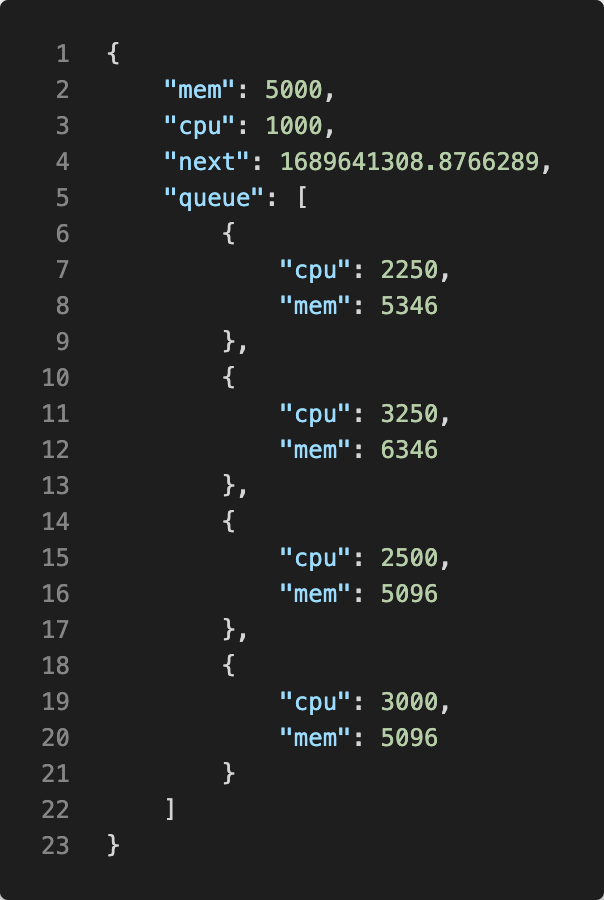
\includegraphics[width=0.45\textwidth]{chapter-4/rc-queue-ex.png}
    \caption{Contoh File Antrian Pengubahan Alokasi}
    \label{fig:ex-queue-rc}
\end{figure}

% TODO CONTOH SISTEM ANTRIAN
\subsection{Komponen \textit{Flexible Control}}

\textbf{\textit{Flexible Control}} mengkolaborasikan \textbf{\textit{Rule Manager}}, \textbf{\textit{Resource Controller}}, \textbf{\textit{Predict Component Factory}} dan \textbf{\textit{Predict Component Storage}}. Komponen ini akan meminta list waktu prediksi yang diperlukan dari \textbf{\textit{Rule Manager}} untuk \textbf{\textit{Rule Manager}} sehingga \textbf{\textit{Predict Component Storage}} dapat menyediakan data prediksi. Setelah itu, semua \textbf{\textit{Rule}} yang memenuhi syarat akan langsung ditransformasikan dan dikirim ke komponen \textbf{\textit{Resource Controller}}. Selain itu, komponen ini juga bertanggung jawab meneruskan data ke \textbf{\textit{Predict Component Storage}} untuk melakukan penambahan data. Spesifikasi kelas ini dapat dilihat pada gambar \ref{fig:ac-spek}.

\begin{figure}[h]
    \centering
    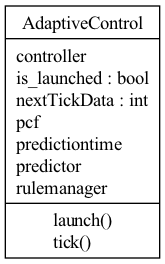
\includegraphics[width=0.3\textwidth]{chapter-4/ac.png}
    \caption{Spesifikasi Kelas Penyusun Komponen \textit{Flexible Control}}
    \label{fig:ac-spek}
\end{figure}
\subsection{Komponen Pendukung: Konfigurasi dan Utilitas}
\label{sec:komponen-pendukung}

Seperti yang sudah dijelaskan sebelumnya, terdapat konfigurasi yang dapat mengatur sistem. Konfigurasi yang dapat diatur dapat dilihat pada gambar \ref{fig:config-spek}.

\begin{figure}[h]
    \centering
    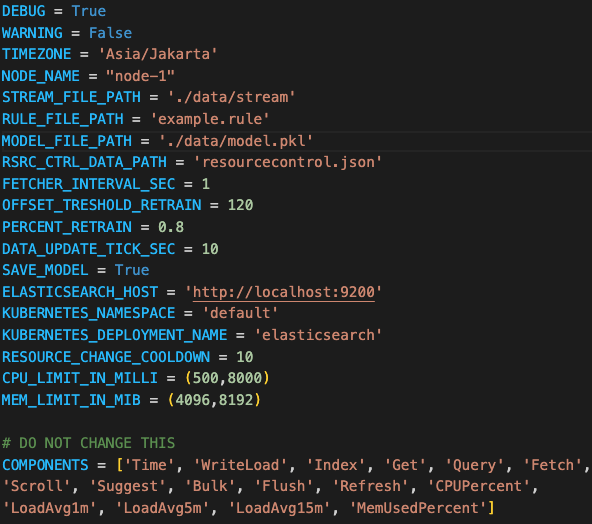
\includegraphics[width=0.8\textwidth]{chapter-4/config.png}
    \caption{Konfigurasi \textit{Flexible Control}}
    \label{fig:config-spek}
\end{figure}

Setiap konfigurasi tersebut mengatur perilaku dari sistem. Untuk setiap konfigurasinya, berikut adalah penjelasannya.

\begin{enumerate}
    \item \textbf{\textit{Debug}} dan \textbf{\textit{Warning}}
    
    Kedua \textit{flag} ini adalah untuk mematikan dan menyalakan pesan \textit{debug} dan \textit{warning}. Jika \textit{debug} dimatikan, maka program tidak akan mengirimkan pesan apapun selama berjalan.

    \item \textbf{\textit{Timezone}}
    
    Flag ini bertujuan untuk mengubah zona waktu yang digunakan oleh pandas karena data yang didapatkan dari \textit{Elastic Search} adalah berupa unix time sehingga akan dibaca secara \textit{default} menjadi UTC saat dikonversi.

    \item \textbf{\textit{Node Name}}, \textbf{\textit{Namespace}} dan \textbf{\textit{Deployment Name}}
    
    \textbf{\textit{Node Name}} adalah nama \textit{node} yang telah dikonfigurasi pada \textit{pods Elastic Search}. Nama harus sesuai karena \textbf{\textit{Metrics Fetcher}} akan mencari data untuk node dengan nama tersebut. Sedangkan, \textbf{\textit{Namespace}} dan \textbf{\textit{Deployment Name}} berkaitan dengan \textit{namespace} dan \textit{deployment Elasticsearch} dengan Kubernetes.

    \item \textbf{\textit{Elasticsearch Host}}
    
    \textit{Flag} ini berisikan target \textit{host} dari \textit{Elasticsearch}. Bertindak sebagai \textit{Base URL} untuk mengakses API \textit{Elastic Search}.

    \item \textbf{\textit{CPU Limit}} dan \textbf{\textit{Memory Limit}}
    
    Kedua limit ini digunakan untuk \textbf{\textit{Resource Controller}} mengubah alokasi sumber daya. \textit{Flag} ini berisikan \textit{tuple} dengan dua buah angka yang berguna sebagai batas bawah dan batas atas dari sumber daya bersangkutan. Satuan yang digunakan untuk prosesor adalah mili (m) sedangkan untuk memori adalah \textit{mebibyte} (MiB). Kedua batas ini bersifat inklusif.

    \item \textbf{\textit{File Path}}
    
    Seperti namanya, konfigurasi yang berkaitan dengan \textit{file path} berfungsi untuk mengatur tata letak file yang akan dibuat/dibaca oleh sistem.

    \item \textbf{\textit{Fetcher Interval}}, \textbf{\textit{Resource Change Cooldown}} dan \textbf{\textit{Data Update Tick Second}}
    
    \textbf{\textit{Fetcher Interval}} adalah interval komponen \textbf{\textit{Metrics Fetcher}} melakukan penarikan data. Lalu, \textbf{\textit{Resource Change Cooldown}} adalah waktu yang diperlukan oleh \textbf{\textit{Resource Controller}} untuk menunggu sebelum melakukan perubahan sumber daya. Terakhir, \textbf{\textit{Data Update Tick Second}} adalah interval yang digunakan oleh \textbf{\textit{Flexible Control}} untuk melakukan pembacaan data dari \textit{stream file}. \textbf{\textit{Data Update Tick Second}} harus lebih besar sama dengan \textbf{\textit{Fetcher Interval}} agar efisien. Satuan yang digunakan oleh ketiga \textit{flag} tersebut adalah detik.

    \item \textbf{\textit{Save Model}}
    
    \textit{Flag} ini berfungsi untuk mematikan penyimpanan model setiap kali model berubah. Jika \textit{flag} ini tidak dinyalakan, maka setiap kali sistem melakukan \textit{restart}, model prediksi akan diulang dari kosong.

    \item \textbf{\textit{Offset Treshold Retrain}} dan \textbf{\textit{Percent Retrain}}
    
    Dalam melakukan penambahan data, tidak setiap saat model akan di-\textit{retrain}. Saat tidak di-\textit{retrain}, model prediksi hanya melakukan update yang jauh lebih cepat namun tidak terlalu akurat. Terdapat sebuah angka yang akan menentukan kapan model harus di-\textit{retrain}. Hal ini diperlukan karena melakukan \textit{retrain} membutuhkan waktu yang lama terutama saat data sudah sangat besar. \textbf{\textit{Offset Treshold Retrain}} adalah angka yang menentukan kapan model harus di-\textit{retrain} berdasarkan jumlah data fixed. Sedangkan, \textbf{\textit{Percent Retrain}} adalah angka yang menentukan kapan model harus di-\textit{retrain} berdasarkan persentase jumlah data saat itu. Dengan persamaan \ref{eq:retrain-time}, \textbf{\textit{Offset Treshold Retrain}} adalah variable $c$ dan \textbf{\textit{Percent Retrain}} adalah variable $p$.
\end{enumerate}

Terdapat juga fungsi-fungsi utilitas yang akan membantu komponen-komponen yang telah dijelaskan sebelumnya, spesifikasi utilitas bisa dilihat pada gambar \ref{fig:util-spek}. Untuk setiap fungsinya, berikut adalah kegunaannya.

\begin{enumerate}
    \item \textbf{\textit{Save Model}}
    
    Fungsi ini akan menyimpan model yang telah dilatih ke dalam sebuah file. Digunakan kakas \textit{pickle} untuk melakukan hal ini.

    \item \textbf{\textit{Load Model}}
    
    Fungsi ini akan memuat model yang telah dilatih dari sebuah file. Digunakan kakas \textit{pickle} untuk melakukan hal ini.

    \item \textbf{\textit{Timings}}
    
    Fungsi adalah abstraksi untuk menghitung waktu eksekusi. Digunakan fungsi sebagai \textit{return value} agar lebih rapih ketika diperlukan banyak penghitungan waktu eksekusi.

    \item \textbf{\textit{Printd}}
    
    Fungsi ini hanyalah \textit{wrapper} dari fungsi \textit{print} pada Python untuk mengikuti aturan konfigurasi.

    \item \textbf{\textit{Read From File}}
    
    Fungsi ini digunakan untuk membaca \textit{stream file}. Fungsi ini digunakan oleh komponen \textbf{\textit{Flexible Control}} untuk membaca secara periodik, mentranformasikan dan mengirimkan data ke \textbf{\textit{Predict Component Storage}}.

    \item \textbf{\textit{To Vector}}
    
    Fungsi ini adalah fungsi transformasi format JSON (\textit{Java Syntax Object Notation}) yang ditulis ke \textit{stream file} menjadi sebuah \textit{numpy array} yang akan digunakan untuk membuat \textit{pandas dataframe}.

    \item \textbf{\textit{Create Dataframe}}
    
    Seperti namanya, fungsi ini membuat dataframe dari data yang telah dibaca dari \textit{stream file} dan sudah ditransformasikan dengan fungsi \textbf{\textit{to vector}}.

    \item \textbf{\textit{Extract Number From String}}
    
    Fungsi ini memanfaatkan regex untuk mengambil angka dari sebuah string.
\end{enumerate}

\begin{figure}[h]
    \centering
    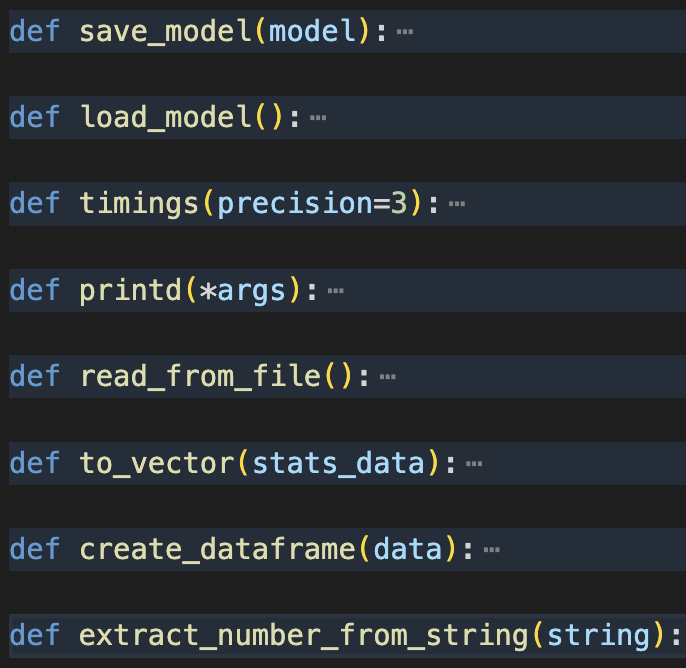
\includegraphics[width=0.6\textwidth]{chapter-4/utils.png}
    \caption{Spesifikasi Fungsi Utilitas Pendukung}
    \label{fig:util-spek}
\end{figure}